\documentclass{beamer}
\usetheme{metropolis} % Use metropolis theme

\title{ECON 3818: Introduction to Statistics with Computer Applications}
%\subtitle
\date{\today}
\author{Kyle Butts}

\definecolor{blue}{RGB}{0,114,178}
\definecolor{red}{HTML}{EB0E09}
\definecolor{yellow}{RGB}{240,228,66}
\definecolor{green}{RGB}{0,158,115}
\definecolor{maroon}{HTML}{AF3335}
\definecolor{purple}{HTML}{7E90B8}

\definecolor{mybackground}{HTML}{ECECEC}
\setbeamercolor{background canvas}{bg= mybackground}

\definecolor{buff-gold}{HTML}{CFB87C}
\definecolor{buff-grey}{HTML}{565A5C}
\definecolor{buff-lightgrey}{HTML}{A2A4A3}
\definecolor{buff-black}{HTML}{000000}

\setbeamercolor{alerted text}{fg=buff-gold!80!black}
\setbeamercolor{frametitle}{bg=buff-black}
\setbeamercolor{title}{fg=buff-grey}
\setbeamercolor{button}{bg=buff-gold}

% Allow to remove indent w/ \begin{itemize}[leftmargin= *]
\usepackage{enumitem}
\setlist[itemize]{label= \textbullet}

% \usepackage[libertine]{newtxmath}
\usepackage{longtable}
\usepackage{booktabs}
\usepackage{enumitem}


\begin{document}

% Title Page ---------------------------------------
\maketitle




% Chapter 17 ---------------------------------------
\section{Chapter 17: Tests for Significance}

\begin{frame}{Outline}
	Things to cover in Chapter 17: 
	\begin{itemize}
		\item Reason we test for significance
		\item Stating a hypothesis
		\item p-value and statistical significance
		\item Tests for a population mean
	\end{itemize}
\end{frame}

\begin{frame}{Statistical Inference}
	
	Two most common types of statistical inference
	\begin{itemize}
		\item Confidence interval
		      \begin{itemize}
		      	\item when the goal is to estimate a population parameter
		      \end{itemize}
		\item Tests of significance
		      \begin{itemize}
		      	\item asses the evidence provided by data about a claim concerning the population
		      \end{itemize}
	\end{itemize}
	
\end{frame}

\begin{frame}{Tests of Significance}
	
	\alert{Definition}: Formal procedure for comparing observed data with a claim (hypothesis) whose truth we want to assess

	Basic idea: an outcome that would rarely happen if a certain claim is true, is good evidence that that claim is not true 
	
\end{frame}

\begin{frame}{Example}
	Suppose that the return on Spotify stock is normally distributed with an unknown mean and a variance $\sigma^2=1$. 
	
	You measure gains and losses for 10 trading days and collect the following sample:
	$$1.6, 0.4, -2.5, 1.5, -1.1, 1.3, -0.1, -0.3, 1.2$$
	The average rate of return is $\bar{X}=0.3$, but there are quite a few days with losses.
\end{frame}

\begin{frame}{Example}
	
	In hypothesis testing, we proceed under the assumption our claim is true and then try to disprove it
	
	For example we could claim $\mu=0$, that is the average Spotify return is 0\%.
	
	Since the data are drawn from a normal distribution, the sample mean is distributed $\bar{X} \sim N(0, \frac{1}{10})$
	
	Now we can use the sampling distribution to comment on how unlikely this claim is. 
	
\end{frame}

\begin{frame}{Example}
	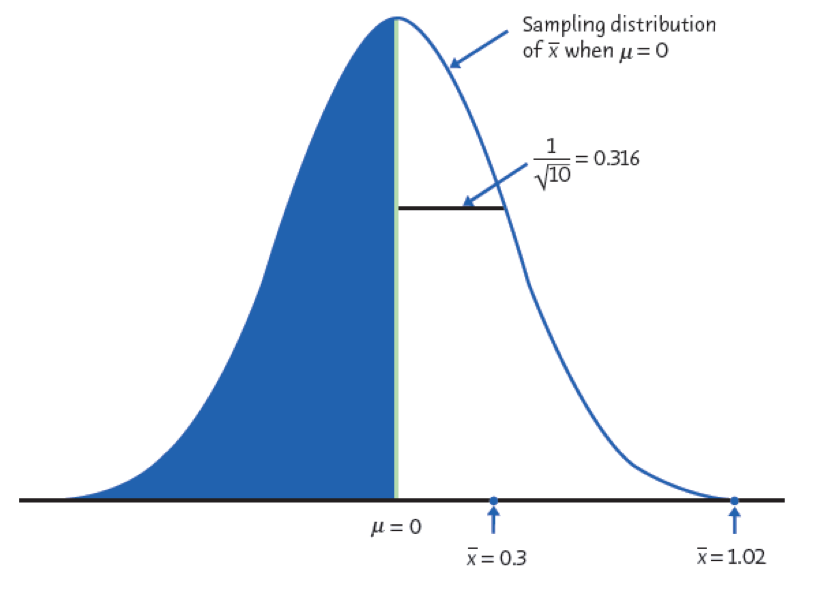
\includegraphics[width=\textwidth]{nullhypothesisdistn}
\end{frame}

\begin{frame}{Stating a Hypothesis}
	
	It is very important to state the hypothesis clearly. 
	\vskip.25in
	A hypothesis has two parts
	\begin{itemize}
		\item \alert{Null hypothesis}, denoted $H_0$, is the claim we are trying to disprove
		      \begin{itemize}
		      	\item test is designed to test the strength of evidence against the null hypothesis 
		      \end{itemize}
		\item \alert{Alternative hypothesis}, denoted $H_1$, is the claim we are trying to find evidence for
		      \begin{itemize}
		      	\item antithesis of the null
		      	      
		      \end{itemize}
	\end{itemize}
\end{frame}

\begin{frame}{Alternative Hypothesis}
	
	There are two types of alternative hypotheses
	
	\begin{itemize}
		\item One-sided alternative
		      \begin{itemize}
		      	\item states the parameter is either larger \textbf{or} smaller 
		      \end{itemize}
		      
		\item Two-sided alternative
		      \begin{itemize}
		      	\item simply states the parameter is \textit{different} from the null
		      \end{itemize}
	\end{itemize}
	
\end{frame} 

\begin{frame}{Example}
	
	Back to the Spotify example:
	
	Lets say we're claiming there is no return on average. We would like to see if we can disprove this hypothesis in favor of a claim that there is a positive return
	$$H_0: \mu=0$$
	$$H_1: \mu > 0$$
	
	\textbf{Clicker Question}: What type of hypothesis test is this?
	\begin{enumerate}[label=(\alph*)]
		\item alternative
		\item null
		\item one-sided
		\item two-sided
	\end{enumerate}
	
\end{frame}

\begin{frame}{Continuing Example}
	So in the Spotify example, we had 10 observations with a sample mean, $\bar{X}=0.3$. We also somehow know that $\sigma^2 = 1$. 
	
	If we want to test the hypothesis 
	$$H_0: \mu=0$$
	$$H_1: \mu > 0$$

	We want to calculate the probability we got an $\bar{X}$ as extreme as 0.3 if the true population $\mu=0$. This means we want to calculate $P(\bar{X}>0.3)$ if $\bar{X} \sim N(0,\frac{1}{10})$

\end{frame}

\frame{}

\begin{frame}{Continuing Example}
	So in the Spotify example, we had 10 observations with a sample mean, $\bar{X}=0.3$. We also somehow know that $\sigma^2 = 1$. 
	
	If we want to test the hypothesis 
	$$H_0: \mu=0$$
	$$H_1: \mu > 0$$

	We want to calculate the probability we got an $\bar{X}$ as extreme as 0.3 if the true population $\mu=0$. This means we want to calculate $P(\bar{X}>0.3)$ if $\bar{X} \sim N(0,\frac{1}{10})$

	$$P(\bar{X}>0.3) = P(\frac{\bar{X}-\mu}{\sigma/\sqrt{n}} > \frac{0.3-\textbf{0}}{1/\sqrt{10}}) = P(Z>0.95) = 0.1711$$
\end{frame}


\begin{frame}{p-Values}
	
	\textbf{Definition of p-value:} Suppose you calculate a test statistic $\hat{\theta}$ from the data, and formulate a null hypothesis $H_0: \theta=\theta_0$ about the true value of $\theta$
	\begin{itemize}
		\item \alert{p-value} is the probability that the test statistic takes a value as or more extreme than the observed value $\hat{\theta}$, \textbf{under the assumption that $H_0$ is true} ($\theta=\theta_0$)
	\end{itemize}
	
	In general, the test statistic we calculate is $\bar{X}$ and formulate a hypothesis about $\mu$
	\begin{itemize}
		\item In this context, the p-value is the probability of getting an $\bar{X}$ so extreme, if the true population mean is equal to $\mu$
	\end{itemize}
	
\end{frame}


\begin{frame}{Calculating p-values}
	
	The way a p-value is calculated changes depending on the type of alternative hypothesis we have:
	$$H_1: \mu> \mu_0, \text{\hspace{10mm}} p = P(\bar{X} \geq \bar{X}_{obs} \big\vert \mu=\mu_0)$$
	
	$$H_1: \mu< \mu_0, \text{\hspace{10mm}} p = P(\bar{X} \leq \bar{X}_{obs} \big\vert \mu=\mu_0)$$
	
	$$H_1: \mu \neq \mu_0, \text{\hspace{10mm}} p = 2 \cdot P(\bar{X} \geq \vert\bar{X}_{obs} \vert  \big\vert  \mu=\mu_0)$$

	where $\bar{X}$ is a random variable, and $\bar{X}_{obs}$ is our observed value for the sample statistic.
	
\end{frame}

\begin{frame}{Example -- One-sided}
	Lets say we have a sample of 30 observations and calculate a sample mean of 1020. We also know that the standard deviation is $\sigma=40$. We want to test the following hypothesis:
	$$H_0: \mu=1000$$
	$$H_1: \mu > 1000$$

	$$p = P(\bar{X} \geq 1020 \ \big| \ \mu=1000)$$
	
\end{frame}

\frame{}

\begin{frame}{Example -- One-sided}
	Lets say we have a sample of 30 observations and calculate a sample mean of 1020. We also know that the standard deviation is $\sigma=40$. We want to test the following hypothesis:
	$$H_0: \mu=1000$$
	$$H_1: \mu > 1000$$
	
	$$p=P(\bar{X} \geq  1020 \ \big| \  \mu=1000)$$
	$$P(\frac{\bar{X}-\mu_0}{\sigma/\sqrt{n}}\geq \frac{1020-1000}{40/\sqrt{30}} )= P(Z>2.74)=0.0032$$
	
	So $p=0.003$, the probability we get a sample mean as large as 1020 if the true mean is 1000 is .3\%
\end{frame}

\begin{frame}{Example -- Two-sided}
	Say we have nine observations, and calculate a sample mean of $\bar{X}$=0.5. We know the underlying distribution has a standard deviation $\sigma=1$. We want to test the following hypothesis:
	$$H_0: \mu=0$$
	$$H_1: \mu \neq 0$$

	$$p=2 \cdot P(\bar{X} \geq 0.5 \ \big| \ \mu=0)$$
	
\end{frame}

\frame{}

\begin{frame}{Example -- Two-sided}
	Say we have nine observations, and calculate a sample mean of $\bar{X}$=0.5. We know the underlying distribution has a standard deviation $\sigma=1$. We want to test the following hypothesis:
	$$H_0: \mu=0$$
	$$H_1: \mu \neq 0$$
	
	$$p=2 \cdot P(\bar{X} \geq 0.5 \ \big| \ \mu=0)$$
	$$2 \cdot P(\frac{\bar{X}-\mu_0}{\sigma/\sqrt{n}}\geq \frac{0.5-0}{1/\sqrt{9}} )=2 \cdot P(Z>1.5)=2\cdot(0.067)=0.134$$
	
	So $p=0.134$, meaning there is a 13.4\% probability of getting a sample mean as far away as 0.5 if the true mean is 0.
\end{frame}



\begin{frame}{Breakout Group}
	Say we have a sample of 25 observations and we calculate a sample mean of 11,500. We know that the standard deviation is $\sigma=5000$. We want to test the following hypothesis:
	$$H_0: \mu=12,675$$
	$$H_1: \mu < 12,675$$
	
	Calculate the p-value:
	\begin{enumerate}[label=(\alph*)]
		\item 0.407
		\item 0.814
		\item 0.119
		\item 0.238
	\end{enumerate}
\end{frame}

\frame{}

\begin{frame}{Hypothesis Testing}
	\footnotesize{ A restaurant owner is determining whether to expand her restaurant to another location. She counts the number of customers per weekend and calculates an average of 538 customers over 50 weekends. She's heard that restaurants of her size shouldn't expand unless they get more than 510 customers each weekend. Conduct a hypothesis at the $\alpha=0.05$ level and determine whether or not she can feel confident she gets at least 510 customers each weekend. Assume $\sigma= 120$.
		\begin{itemize}
			\item State Null \& Alternative hypotheses
			\pause
			      \begin{itemize}
			      	\item $H_0: \mu=510$
			      	\item $H_1: \mu \geq 510$
			      \end{itemize}
			\item Calculate p-value
			\pause
			      \begin{itemize}
			      	\item $P(\bar{X} \geq 538 | \mu=510)=0.049$
			      \end{itemize}
		\end{itemize}}
	Interpretation of p-value: 
	\pause If true population mean is 510, there is a 4.95\% probability of calculating a sample mean as large as 538
\end{frame}

\begin{frame}{Interpreting p-Values}
	Small p-values are evidence against the null, because they say \textbf{the observed value of the sample statistic if very unlikely to occur if the null hypothesis, $H_0$, is true.} 
	\vskip.25in
	Larger p-values fail to give evidence against the null because the observed sample statistic could have resulted by chance if the null hypothesis, $H_0$ is true. 
	\vskip.25in
	
	\pause
	\Large{p-values \alert{DO NOT} tell you the probability that $H_0$ is true!!}
\end{frame}


\begin{frame}{p-Values and Statistical Significance}
	To review, our decision process using p-values is
	\begin{itemize}
		\item p-value is sufficiently small $\rightarrow$ reject $H_0 \rightarrow$ accept $H_1$
		\item p-value is too large $\rightarrow$ fail to reject $H_0 \rightarrow$ do not accept $H_1$
	\end{itemize}

	We \textbf{never} say "accept $H_0$". All we can say is if there is enough evidence to say it is false, we cannot know for certain if it is true.
	
	\pause
	\Large{We say our results are \alert{statistically significant} if we reject $H_0$}
\end{frame}

\begin{frame}{p-Values and Statistical Significance}
	How small does p need to be in order to be "sufficiently small"? When can we claim our results are statistically significant?
	\vskip.25in
	Suppose you calculate a p-value, and specify a \alert{level of significance}, $\alpha$. We say our results are \alert{statistically significant} if:
	$$\text{p-value} \leq \alpha$$
	
	We will discuss how to correctly specify $\alpha$. Some of the most common levels of significance are .01, .05, and 0.1. 
\end{frame}


\begin{frame}{Example}
	\footnotesize{A restaurant owner is determining whether to expand her restaurant to another location. She counts the number of customers per weekend and calculates an average of 538 customers over 50 weekends. She's heard that restaurants of her size shouldn't expand unless they get more than 510 customers each weekend. Conduct a hypothesis at the $\alpha=0.05$ level and determine whether or not she can feel confident she gets at least 510 customers each weekend. Assume $\sigma= 120$.
		\begin{itemize}
			\item State Null \& Alternative hypotheses
			      \begin{itemize}
			      	\item $H_0: \mu=510$
			      	\item $H_1: \mu \geq 510$
			      \end{itemize}
			\item Calculate p-value
			      \begin{itemize}
			      	\item $P(\bar{X} \geq | \mu=510)=0.049$
			      \end{itemize}
			\item Compare p-value to 0.05
			      \begin{itemize}
			      	\item $0.049 < 0.05 \rightarrow p-value<\alpha \rightarrow$ Reject $H_0$
			      \end{itemize}
		\end{itemize}
	Reject null hypothesis in favor of alternative, that the true population mean number of customers is greater than 510}
\end{frame}

\begin{frame}{Hypothesis Testing Algorithm}
	
	A hypothesis test consists of 5 parts
	
	\begin{itemize}
		\item Null hypothesis, $H_0$
		\item Alternative hypothesis, $H_1$
		\item Test statistic, $\hat{\theta}$, most commonly $\bar{X}$
		\item Rejection region, $\text{p-value}\leq \alpha$
		\item Conclusion
		      \begin{itemize}
		      	\item reject $H_0$ if $p \leq \alpha$
		      	\item fail to reject $H_0$ if $p > \alpha$
		      \end{itemize}
	\end{itemize}
	
\end{frame}


\begin{frame}{Rejection Region}
	We call the range of values for which we would reject the null the \alert{rejection region}
	
	Calculate rejection region using
	\begin{itemize}
		\item the population mean, $\mu$ under the null hypothesis
		\item the standard deviation, $\sigma$
		\item level of significance, $\alpha$ and Z-score associated it with it
	\end{itemize}
	
	The rejection region tells us how extreme the sample mean needs to be for us to reject the null  hypothesis $H_0: \mu=\mu_0$
	\begin{itemize}
		\item Tells us all the $\bar{X}$'s with a p-value less than $\alpha$
	\end{itemize}
\end{frame}


\begin{frame}{Calculate Rejection Region--One-Sided}
	Let's say we want to test a hypothesis about the number of children in a family. We have a sample of 25 observations, and we know $\sigma=0.8$. We decide to test the following hypothesis:
	$$H_0:\mu=2$$
	$$H_1:\mu<2$$
	If we are testing at the 5\% significance level, calculate the rejection region. 
	\begin{itemize}
		\item The rejection region is the values of $\bar{X}$ that are far enough away from $\mu$ that we would reject $H_0$
		\item We want to find $\bar{X}^*$ that solves 
		
		$$R = P(\bar{X} \leq \bar{X}^* \vert \mu_0 =2) = 0.05$$
	\end{itemize}
\end{frame}

\frame{}
\frame{}

\begin{frame}{Calculating Rejection Region--One-Sided}
	$$P(\bar{X}\leq\bar{X}^* \vert \mu_0 = 2)=0.05=P(Z\leq\frac{\bar{X}^*-\mu}{\sigma/\sqrt{n}})$$
	$$P(Z\leq\frac{\bar{X}^*-2}{0.8/5})=0.05=P(Z\leq\frac{\bar{X}^*-2}{.16})=0.05$$
	
	We know that $P(Z \leq -1.645)=0.05$, therefore:
	$$\frac{\bar{X}^*-2}{0.16}=-1.645 \rightarrow \bar{X}^*=1.74$$
	This means our rejection region is all $\bar{X}\leq1.74$. In words, we will reject $H_0:\mu=2$ at the $\alpha=0.05$ level if we calculate a sample mean of 1.74 or smaller.
	
\end{frame}

\begin{frame}{Breakout Group}
	A study is conducted to determine the average income of 18-25 year olds in San Antonio. They are trying to test whether the average is greater than \$21,000. The study is able to collect 16 different salaries. We somehow know that the population standard deviation is $\sigma=$\$2000. What sample averages would we reject the null hypothesis at the $\alpha=0.05$ level?
	$$H_0: \mu=\$21,000$$
	$$H_1: \mu > \$21,000$$
	\begin{enumerate}[label=(\alph*)]
		\item Reject if $\bar{X} < \$21,822.5$
		\item Reject if $\bar{X} > \$21,822.5$
		\item Reject if $\bar{X} < \$20,177.5$
		\item Reject if $\bar{X} >\$20,177.5$
	\end{enumerate}
\end{frame}

\begin{frame}{Calculating Rejection Region--Two-Sided}
	Solving for a rejection region changes a little bit when we consider a two-tailed test.
	
	Example: Suppose we have a sample of 25 observations, we know $\sigma=3.5$. We want to test the following hypothesis at the $\alpha=0.05$ level. 

	$$H_0: \mu=13.5$$
	$$H_1: \mu \neq 13.5$$

	Our rejection region is calculated by finding two different $\bar{X}^*$'s.

	$$P(\bar{X}\geq\bar{X}^*_U)=\frac{0.05}{2}$$
	$$P(\bar{X}\leq\bar{X}^*_L)=\frac{0.05}{2}$$

\end{frame}

\frame{}
\frame{}

\begin{frame}{Calculating Rejection Region -- Two-Sided}
	$$P(\bar{X}\geq\bar{X}^*_U)= \frac{0.05}{2} = 0.025 = P(Z>\frac{\bar{X}^*_U-13.5}{0.64})$$
	\begin{itemize}
		\item  We know $P(Z>1.96)=0.025$. 
		
		\item Therefore: $$\frac{\bar{X}^*_U-13.5}{0.64}=1.96 \implies \bar{X}^*_U=14.75$$
	\end{itemize}
\end{frame}

\begin{frame}{Breakout Group}
	For the same problem, solve for $\bar{X}^*_L$.
	
	\vspace{5mm}
	Remember it solves: $P(\bar{X}\leq\bar{X}^*_L)=\frac{0.05}{2}$
	
	\begin{enumerate}[label=(\alph*)]
		\item -14.75
		\item 12.246
		\item 11.54
	\end{enumerate}
\end{frame}

\frame{}

\begin{frame}{Solving Hypothesis Testing Problem}
	\begin{itemize}
		\item p-Value method
		      \begin{itemize}
		      	\item calculate p-value, varies based off type of alternative hypothesis
		      	\item p-value: probability of getting as extreme of a sample statistic, if the null hypothesis is true
		      	\item compare p-value with level of significance $\alpha$
		      	      \begin{itemize}
		      	      	\item if $p<\alpha \rightarrow$, reject $H_0$
		      	      \end{itemize}
		      \end{itemize}
		\item Rejection region method
		      \begin{itemize}
		      	\item calculate rejection region based off level of significance
		      	\item compare sample statistic with rejection region
		      	      \begin{itemize}
		      	      	\item if sample statistic is in rejection region, reject $H_0$
		      	      \end{itemize}
		      \end{itemize}
	\end{itemize}
\end{frame}




\end{document}